\documentclass[conference]{IEEEtran}
\IEEEoverridecommandlockouts

\usepackage{amsmath,amssymb,amsfonts}
\usepackage{algorithmic}
\usepackage{graphicx}
\usepackage{textcomp}
\usepackage{xcolor}
\usepackage{biblatex}
\addbibresource{refs.bib}

\def\BibTeX{{\rm B\kern-.05em{\sc i\kern-.025em b}\kern-.08em
    T\kern-.1667em\lower.7ex\hbox{E}\kern-.125emX}}
    
\begin{document}

\title{Maze Escape Robot for BPC-PRP}

\author{\IEEEauthorblockN{Stanislav Doubravský}
\IEEEauthorblockA{\textit{Fakulta elektrotechniky a komunikačních technologií} \\
\textit{Vysoké učení technické v Brně}\\
Brno, Czech Republic \\
256274@vutbr.cz}
\and
\IEEEauthorblockN{Jan Grulich}
\IEEEauthorblockA{\textit{Fakulta elektrotechniky a komunikačních technologií} \\
\textit{Vysoké učení technické v Brně}\\
Brno, Czech Republic \\
256285@vutbr.cz}
}

\maketitle

\begin{abstract}
This project focuses on the implementation of an autonomous mobile robot designed for the final “Maze Escape” task in the course BPC-PRP (Practical Robotics and Computer Vision). The robot is based on a differential drive platform equipped with LiDAR, IMU, line sensors, wheel encoders, and a camera. The software architecture was implemented in C++ using ROS2 and is divided into modular nodes responsible for sensing, filtering, estimation, and control.

The main objective of the project was to create a robust navigation system capable of following corridors, detecting intersections, recognizing visual navigation hints using ArUco markers, and performing stable turns in a maze environment. Particular attention was paid to real-time sensor fusion, modular software design, and reliable control loops suitable for noisy sensor measurements and imperfect mechanical properties of the robot.

The resulting solution combines several robotics concepts taught during the semester, including PID regulation, odometry, inertial integration, LiDAR processing, finite state machines, and computer vision.
\end{abstract}

\begin{IEEEkeywords}
Robotics, project, BPC-PRP, state-of-the-art
\end{IEEEkeywords}


\section{Introduction}

Autonomous navigation in unknown or semi-structured environments is one of the fundamental problems in mobile robotics. Even relatively simple maze environments introduce multiple practical challenges, including noisy sensor measurements, imperfect localization, unstable control loops, and mechanical inaccuracies of the robot platform.

The goal of this project was to design and implement a fully autonomous robot capable of navigating through a maze environment while reacting to visual navigation hints and maintaining stable movement inside corridors. The project was developed as part of the BPC-PRP course and combines multiple robotics disciplines into a single integrated system.

The implemented robot uses several sensing modalities simultaneously:\newline
- LiDAR for corridor detection and distance estimation\newline
- IMU for orientation tracking and turning stabilization\newline
- Wheel encoders for odometry feedback\newline
- Reflective line sensors for line following\newline
- Camera for ArUco marker recognition

The complete software solution was implemented using ROS2 and modular C++ nodes. The modular architecture allowed independent testing of individual subsystems and simplified debugging during development.

\begin{figure}[h]
    \centering
    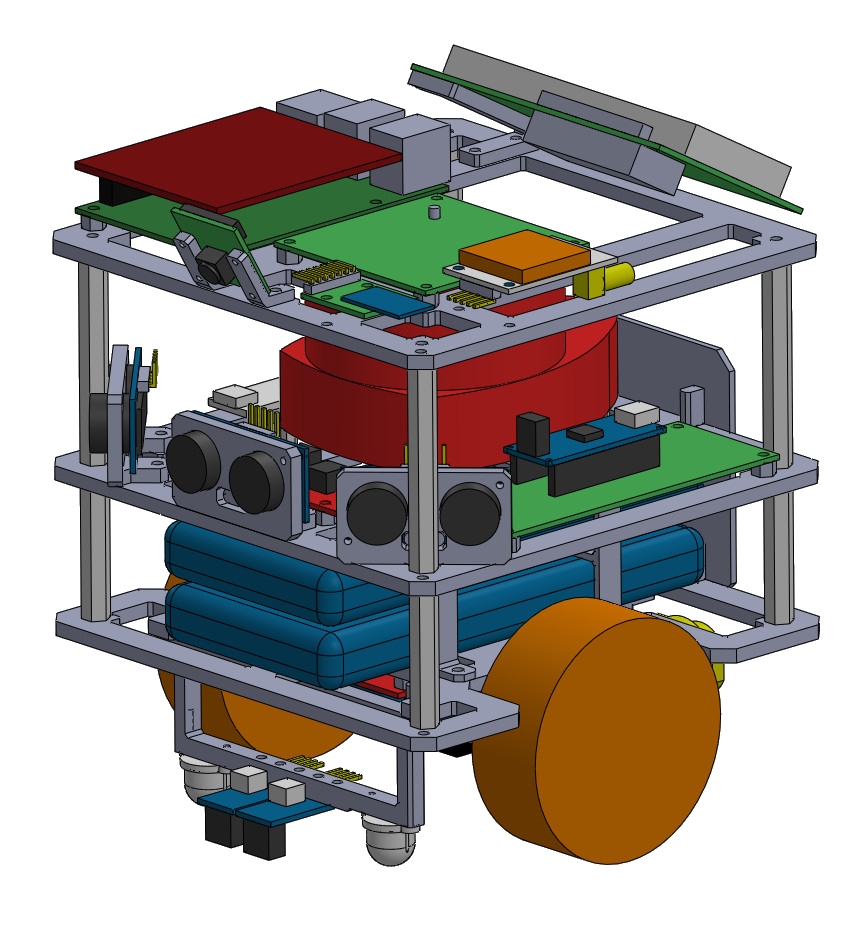
\includegraphics[width=0.45\textwidth]{images/render.png}
    \caption{Implemented autonomous robot platform [3]}
    \label{fig:robot}
\end{figure}


\input{texts/2_method.tex}
\input{texts/3_conclusion.tex}


\section*{Acknowledgment}
Sources and course materials: \newline
[1] BPC-PRP Course Documentation: \newline
-  \url{https://robotics-but.github.io/BPC-PRP} \newline
[2] BPC-PRP Project Template Repository: \newline
-  \url{https://github.com/Robotics-BUT/BPC-PRP} \newline
[3] Fenrir Project Robot Documentation: \newline
-  \url{https://robotics-but.github.io/fenrir-project}

\printbibliography

\end{document}
